\section{Auswertung}
\subsection{Einfachspalt}
Es soll die Spaltbreite ermittelt werden, indem die Aperturfunktion der Blende
auf das Beugungsbild zurückgeführt wird. Das Intensitätsmuster des Beugungsbildes
wurde punktweise aufgenommen, die Messwerte dazu befinden sich in \autoref{tab:10}.
Die Ausgleichsfunktion nach \autoref{eqn:11} ist \autoref{abb:10} zu entnehmen.
\begin{equation}
    \label{eqn:11}
    I\left(\Phi\right) = A^2 \cdot \text{sinc}^2\left(b \cdot \Phi\right) 
\end{equation}
\noindent Durch die Ausgleichsrechnung ergeben sich folgende Parameter:
\begin{align}
    \text{A} = & \qty{0.7156(0.0015)}{\micro\ampere} \\
    \text{b} = & \qty{216.03(0.94)}{\micro\meter}
\end{align}
Dabei gibt der Parameter $b$ die Breite des Spaltes an an dem das Licht gebeugt
wurde. Somit beträgt die experimentell ermittelte breite des Spaltes 
$\qty{0.216(0.0094)}{\milli\meter}$.
\begin{table}[H]
    \centering
    \caption{Messwerte der Intensitätsverteilung des Einfachspalts.}
    \label{tab:10}
    \begin{tblr}{
        colspec = {S S | S S | S S | S S},
        row{1} = {guard, mode=math},}
           \toprule
            \text{x}/ \unit{\milli\meter} & \text{I}/ \unit{\micro\ampere}& \text{x} /\unit{\milli\meter} & \text{I} /\unit{\micro\ampere}& \text{x} /\unit{\milli\meter} & \text{I} /\unit{\micro\ampere} & \text{x} /\unit{\milli\meter} & \text{I}/ \unit{\micro\ampere}\\
           \midrule
           -25   &0.002 +- 0.002& -7      & 0.012   +- 0.002& 4   & 0.060 +- 0.002&20 &0.002 +- 0.002\\              
           -24   &0.002 +- 0.002& -6.5    & 0.008   +- 0.002& 4.5 & 0.040 +- 0.002&21 &0.002 +- 0.002\\    
           -23   &0.000 +- 0.002& -6      & 0.006   +- 0.002& 5   & 0.014 +- 0.002&22 &0.000 +- 0.002\\    
           -22   &0.000 +- 0.002& -5.5    & 0.010   +- 0.002& 5.5 & 0.006 +- 0.002&23 &0.000 +- 0.002\\    
           -21   &0.002 +- 0.002& -5      & 0.020   +- 0.002& 6   & 0.004 +- 0.002&24 &0.002 +- 0.002\\    
           -20   &0.002 +- 0.002& -4.5    & 0.040   +- 0.002& 6.5 & 0.008 +- 0.002&25 &0.002 +- 0.002\\    
           -19   &0.002 +- 0.002& -4      & 0.090   +- 0.002& 7   & 0.014 +- 0.002& & \\    
           -18   &0.000 +- 0.002& -3.5    & 0.140   +- 0.002& 7.5 & 0.018 +- 0.002& & \\    
           -17   &0.000 +- 0.002& -3      & 0.200   +- 0.002& 8   & 0.020 +- 0.002& & \\
           -16   &0.002 +- 0.002& -2.5    & 0.280   +- 0.002& 8.5 & 0.018 +- 0.002& & \\
           -15   &0.004 +- 0.002& -2      & 0.340   +- 0.002& 9   & 0.016 +- 0.002& & \\
           -14   &0.006 +- 0.002& -1.5    & 0.420   +- 0.002& 9.5 & 0.012 +- 0.002& & \\
           -13   &0.006 +- 0.002& -1      & 0.460   +- 0.002& 10  & 0.008 +- 0.002& & \\
           -12   &0.004 +- 0.002& -0.5    & 0.500   +- 0.002& 11  & 0.002 +- 0.002& & \\    
           -11   &0.002 +- 0.002& 0       & 0.520   +- 0.002& 12  & 0.004 +- 0.002& & \\
           -10.5 &0.004 +- 0.002& 0.5     & 0.500   +- 0.002& 13  & 0.006 +- 0.002& & \\
           -10   &0.006 +- 0.002& 1       & 0.460   +- 0.002& 14  & 0.006 +- 0.002& & \\
           -9.5  &0.010 +- 0.002& 1.5     & 0.400   +- 0.002& 15  & 0.004 +- 0.002& & \\
           -9    &0.014 +- 0.002& 2       & 0.340   +- 0.002& 16  & 0.002 +- 0.002& & \\    
           -8.5  &0.016 +- 0.002& 2.5     & 0.260   +- 0.002& 17  & 0.002 +- 0.002& & \\    
           -8    &0.017 +- 0.002& 3       & 0.200   +- 0.002& 18  & 0.004 +- 0.002& & \\    
           -7.5  &0.016 +- 0.002& 3.5     & 0.120   +- 0.002& 19  & 0.004 +- 0.002& & \\
            \bottomrule
    \end{tblr}
\end{table}

\label{sec:Auswertung}
\begin{figure}[H]    
    \centering
    \caption{Ausgleichsrechnung zur Intensitätsverteilung des Einfachspaltes.}
    \label{abb:10}
    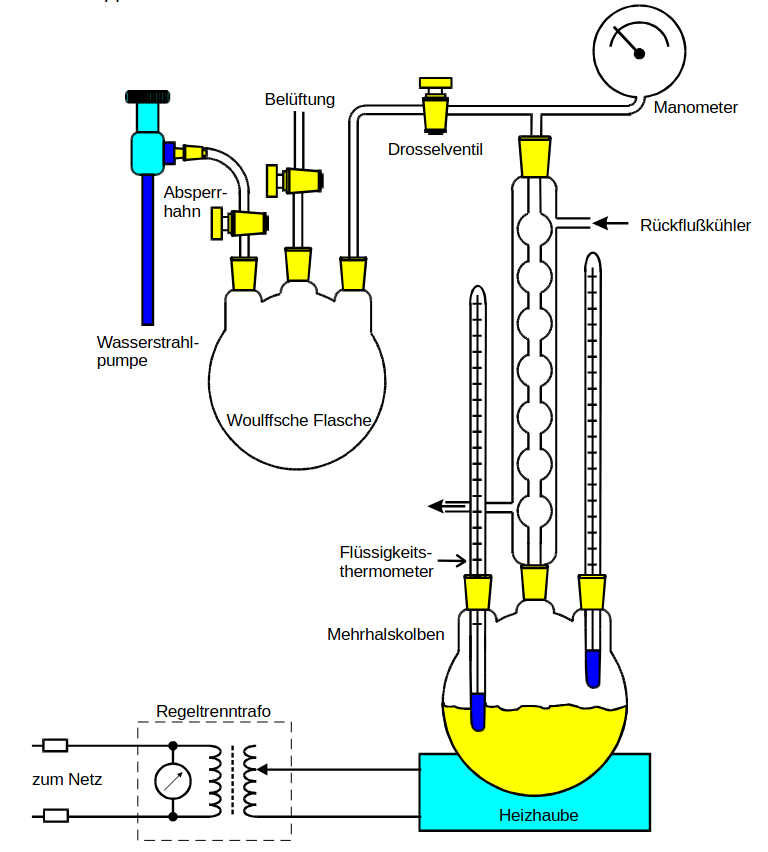
\includegraphics{teil1.pdf}
\end{figure}





\subsection{Doppelspalt}
Ein ähnliches Vorgehen wird bei der Bestimmung der Breite des Doppelspaltes
angewendet. Allerdings wird eine etwas andere Funktion für die Ausgleichsrechnung
verwendet. Diese befindet sich in \autoref{eqn:10}.
\begin{equation}
    \label{eqn:10}
    I\left(\Phi\right) = A^2 \cdot \text{sinc}^2\left(b \cdot \left(x - d\right)\right)  \cdot \cos^2{\left(c \cdot \left(x - d\right)\right)}
\end{equation}
\noindent Die Messdaten der Messung am Doppelspalt befinden sich in \autoref{tab:11}
Die dazugehörige Ausgleichsrechnung ist in \autoref{abb:11} visualisiert.
Die Ausgleichsrechnung durch einen curve Fit des python Paketes scipy ergibt
die Parameter:
\begin{align}
    \text{A} = & \qty{0.6249(0.0078)}{\micro\ampere} \\
    \text{b} = & \qty{121.601(3.079)}{\micro\meter}\\
    \text{c} = & \qty{2809(8)}{} \\
    \text{d} = & \qty{-0.0002(0)}{\milli\meter}
\end{align}
\noindent Daraus ergibt sich für die experimentellen Spaltbreiten des Doppelspalts:
\begin{equation}
    b_\text{Doppelspalt} = \qty{0.12(0.30)}{\milli\meter}.
\end{equation}
\noindent
\begin{table}[H]
    \centering
    \caption{Messwerte der Intensitätsverteilung des Doppelspalts.}
    \label{tab:11}
    \begin{tblr}{
        colspec = {S S | S S | S S | S S},
        row{1} = {guard, mode=math},}
           \toprule
            \text{x}/ \unit{\milli\meter} & \text{I}/ \unit{\micro\ampere}& \text{x} /\unit{\milli\meter} & \text{I} /\unit{\micro\ampere}& \text{x} /\unit{\milli\meter} & \text{I} /\unit{\micro\ampere} & \text{x} /\unit{\milli\meter} & \text{I}/ \unit{\micro\ampere}\\
           \midrule
           -25   & 0.003   +-0.001   &    -8.5        &      0.018   +-0.001     &      0.5    & 0.020   +-0.01     &    9.5    & 0.004    +-0.001   \\              
           -24.5 & 0.002   +-0.001   &    -8.25       &      0.014   +-0.001     &      0.75   & 0.100   +-0.01     &    9.75   & 0.002    +-0.001   \\    
           -24   & 0.001   +-0.001   &    -8          &      0.004   +-0.001     &      1      & 0.300   +-0.01     &    10     & 0.002    +-0.001   \\    
           -23.5 & 0.003   +-0.001   &    -7.75       &      0.010   +-0.001     &      1.25   & 0.400   +-0.01     &    10.5   & 0.004    +-0.001   \\    
           -23   & 0.000   +-0.001   &    -7.5        &      0.030   +-0.001     &      1.5    & 0.240   +-0.01     &    11     & 0.008    +-0.001   \\    
           -22.5 & 0.001   +-0.001   &    -7.25       &      0.056   +-0.001     &      1.75   & 0.060   +-0.01     &    11.5   & 0.004    +-0.001   \\    
           -22   & 0.002   +-0.001   &    -7          &      0.050   +-0.001     &      2      & 0.040   +-0.01     &    12     & 0.004    +-0.001   \\    
           -21.5 & 0.001   +-0.001   &    -6.75       &      0.020   +-0.001     &      2.25   & 0.200   +-0.01     &    12.5   & 0.012    +-0.001   \\    
           -21   & 0.002   +-0.001   &    -6.5        &      0.006   +-0.001     &      2.5    & 0.300   +-0.01     &    13     & 0.004    +-0.001   \\
           -20.5 & 0.003   +-0.001   &    -6.25       &      0.040   +-0.001     &      2.75   & 0.280   +-0.01     &    13.5   & 0.006    +-0.001   \\
           -20   & 0.002   +-0.001   &    -6          &      0.100   +-0.001     &      3      & 0.140   +-0.01     &    14     & 0.012    +-0.001   \\
           -19.5 & 0.002   +-0.001   &    -5.75       &      0.140     +- 0.01   &      3.25   & 0.020   +-0.01     &    14.5   & 0.002    +-0.001   \\
           -19   & 0.001   +-0.001   &    -5.5        &      0.100     +- 0.01   &      3.5    & 0.040   +-0.01     &    15     & 0.006    +-0.001   \\
           -18.5 & 0.001   +-0.001   &    -5.25       &      0.020     +- 0.01   &      3.75   & 0.140   +-0.01     &    15.5   & 0.002    +-0.001   \\    
           -18   & 0.002   +-0.001   &    -5          &      0.020     +- 0.01   &      4      & 0.222   +-0.01     &    16     & 0.003    +-0.001   \\
           -17.5 & 0.001   +-0.001   &    -4.75       &      0.120     +- 0.01   &      4.25   & 0.140   +-0.01     &    16.5   & 0.001    +-0.001   \\
           -17   & 0.000   +-0.001   &    -4.5        &      0.220     +- 0.01   &      4.5    & 0.040   +-0.01     &    17     & 0.002    +-0.001   \\
           -16.5 & 0.002   +-0.001   &    -4.25       &      0.200     +- 0.01   &      4.75   & 0.000   +-0.01     &    17.5   & 0.003    +-0.001   \\
           -16   & 0.006   +-0.001   &    -4          &      0.100     +- 0.01   &      5      & 0.040   +-0.01     &    18     & 0.003    +-0.001   \\    
           -15.5 & 0.006   +-0.001   &    -3.75       &      0.020     +- 0.01   &      5.25   & 0.100   +-0.01     &    18.5   & 0.003    +-0.001   \\    
           -15   & 0.002   +-0.001   &    -3.5        &      0.060     +- 0.01   &      5.5    & 0.100   +-0.01     &    19     & 0.003    +-0.001   \\    
           -14.5 & 0.012   +-0.001   &    -3.25       &      0.240     +- 0.01   &      5.75   & 0.060   +-0.01     &    19.5   & 0.003    +-0.001   \\
           -14   & 0.006   +-0.001   &    -3          &      0.320     +- 0.01   &      6      & 0.020     +-0.001  &    20     & 0.003    +-0.001   \\
           -13.5 & 0.002   +-0.001   &    -2.75       &      0.200     +- 0.01   &      6.25   & 0.000     +-0.001  &    20.5   & 0.003    +-0.001  \\
           -13   & 0.012   +-0.001   &    -2.5        &      0.060     +- 0.01   &      6.5    & 0.040     +-0.001  &    21     & 0.002    +-0.001  \\
           -12.5 & 0.004   +-0.001   &    -2.25       &      0.020     +- 0.01   &      6.75   & 0.060     +-0.001  &    21.5   & 0.003    +-0.001  \\
           -12   & 0.004   +-0.001   &    -2          &      0.140     +- 0.01   &      7      & 0.040     +-0.001  &    22     & 0.002    +-0.001  \\
           -11.5 & 0.006   +-0.001   &    -1.75       &      0.400     +- 0.01   &      7.25   & 0.020     +-0.001  &    22.5   & 0.002    +-0.001  \\
           -11   & 0.002   +-0.001   &    -1.5        &      0.400     +- 0.01   &      7.5    & 0.000     +-0.001  &    23     & 0.003    +-0.001  \\
           -10.5 & 0.002   +-0.001   &    -1.25       &      0.200     +- 0.01   &      7.75   & 0.000     +-0.001  &    23.5   & 0.002    +-0.001  \\
           -10   & 0.004   +-0.001   &    -1          &      0.020     +- 0.01   &      8      & 0.020     +-0.001  &    24     & 0.002    +-0.001  \\
           -9.75 & 0.004   +-0.001   &    -0.75       &      0.060     +- 0.01   &      8.25   & 0.020     +-0.001  &    24.5   & 0.003    +-0.001  \\
           -9.5  & 0.002   +-0.001   &    -0.5        &      0.300     +- 0.01   &      8.5    & 0.000     +-0.001  &    25     & 0.002    +-0.001  \\
           -9.25 & 0.002   +-0.001   &    -0.25       &      0.140     +- 0.01   &      8.75   & 0.000     +-0.001  &       &   \\
           -9    & 0.004   +-0.001   &    0           &      0.360     +- 0.01   &      9      & 0.040     +-0.001  &        &  \\
           -8.75 & 0.012   +-0.001   &    0.25        &      0.140     +- 0.01   &      9.25   & 0.004     +-0.001  &         & \\
        \bottomrule
    \end{tblr}
\end{table}

\begin{figure}[H]
    \centering
    \caption{Ausgleichsrechnung zur Intensitätsverteilung des Doppelspaltes.}
    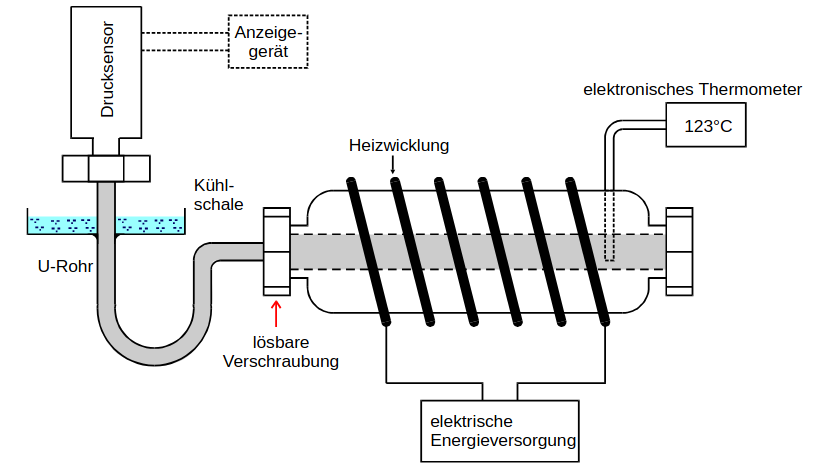
\includegraphics{teil2.pdf}
    \label{abb:11}
\end{figure}

\begin{figure}[H]
    \centering
    \caption{Vergleich der Intensitätsverteilungen Doppelspalt und Einfachspalt.}
    \includegraphics{teil3.pdf}
    \label{abb:12}
\end{figure}


